\documentclass{IMTexam}

\usepackage{IMTtikz}
\DeclareSIUnit{\atm}{atm}
\DeclareSIUnit{\calorie}{cal}
\usepackage{mhchem}

%\mmaDefineMathReplacement[≤]{<=}{\leqslant}
%\mmaDefineMathReplacement[≥]{>=}{\geqslant}
%\mmaDefineMathReplacement[≠]{!=}{\neq}
%\mmaDefineMathReplacement[→]{->}{\to}[2]
%\mmaDefineMathReplacement[⧴]{:>}{:\hspace{-.2em}\to}[2]
%\mmaDefineMathReplacement{∉}{\notin}
%\mmaDefineMathReplacement{∞}{\infty}
%\mmaDefineMathReplacement{𝕕}{\mathbbm{d}}
%\mmaSet{
%  morefv={gobble=2},
%  linklocaluri=mma/symbol/definition:#1,
%  morecellgraphics={yoffset=1.9ex}
%}
\usepackage{listings,xcolor}

\lstset{language=Mathematica}
\lstset{basicstyle={\sffamily\footnotesize},
  numbers=left,
  numberstyle=\tiny\color{gray},
  numbersep=5pt,
  breaklines=true,
  captionpos={t},
  frame={lines},
  rulecolor=\color{black},
  framerule=0.5pt,
  columns=flexible,
  tabsize=2
}


\givecredits
\author{Isabella B. \& Joel B. \& Jonathan B.}
%\USPN{}
\lecture{Química II}
\examname{Prova II}
\hwtype{Resolução}
\lcode{}
\date{12 de julho}

\begin{document}
    \maketitle

    \begin{questions}
        \question Considerando o diagrama de fases ao lado:

        \begin{center}
            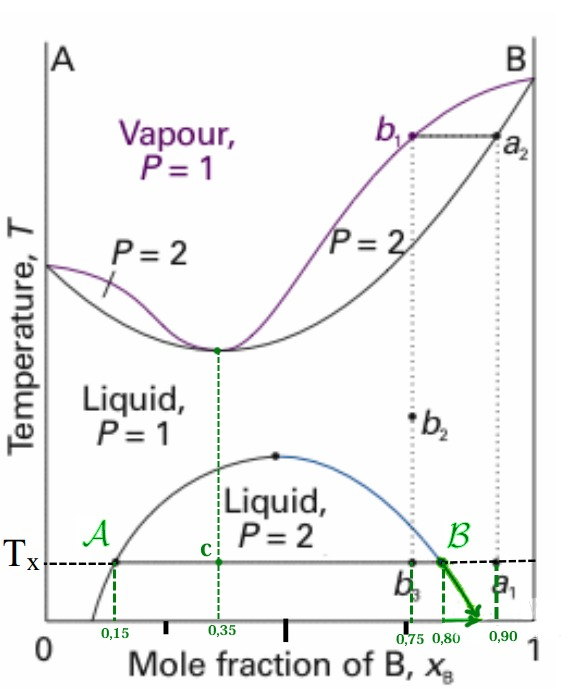
\includegraphics[width=0.5\linewidth]{WhatsApp Image 2021-07-12 at 10.10.58 PM.jpeg}
        \end{center}

        \begin{parts}
            \part Descreva a composição da fase ou das fases representadas
            pelos pontos a1, a2e b3. Inclua estado físico da fase ou das fases
            na sua resposta. No caso de mais de uma fase, inclua a razão em
            mols de uma em relação a outra.

            \begin{solution}
                $a_{1}$ é óbvio: uma única fase líquida de B com A dissolvido.
                Proporção B:A é uns 90:10.

                $a_{2}$ está bem no ponto de ebulição, descrevendo uma fase
                líquida e uma fase gasosa infinitésima. A fase líquida é
                idêntica a $a_{1}$, com \SI{90}{\percent} de B. A fase gasosa é indicada
                pelo ponto $b_{1}$, tendo aprox. \SI{75}{\percent} de B. Não há quase nada
                de gás em cima do ponto de ebulição, então a razão gás/liq é
                quase nula.

                $b_{3}$ descreve duas fases líquidas, nos pontos de intersecção
                entre a sua reta e a curva líquido-líquido. O ponto da
                esquerda, chamemos de $\mathcal{A}$, descreve uma fase com
                aprox. \SI{85}{\percent} de A dissolvendo \SI{15}{\percent} de
                B, enquanto o da direita,
                chamemos de $\mathcal{B}$, descreve uma fase com aprox. \SI{80}{\percent} de
                B dissolvendo \SI{20}{\percent} de A. Pela regra da alavanca, temos
                $\frac{\eta_{\mathcal{A}}}{\eta_{\mathcal{B}}} =
                \frac{l_{\mathcal{B}}}{l_{\mathcal{A}}}$. Considerando
                $l_{\mathcal{B}} \approx 0.05$ e $l_{\mathcal{A}} \approx 0.6$,
                $\frac{\eta_{\mathcal{A}}}{\eta_{\mathcal{B}}} \approx
                \frac{1}{12}$.

            \end{solution}

            \part Suponha que você inicie uma destilação a partir do ponto a1.
            Considerando que a destilação é conduzida até o
            azeótropo de mínimo ser atingido e que o vapor é recolhido e
            condensado a mesma temperatura que a destilação começou
            (Tx), determine a composição da fase ou das fases que você vai
            obter após a destilação.

            \begin{solution}
                O ponto c no gráfico indica o ponto onde os destilados serão
                recolhidos. Por análise similar à feita para $b_{3}$ no último
                item, vemos que duas fases serão geradas: $\mathcal{A}$ de A:B
                85:15 e $\mathcal{B}$ de A:B 20:80. Por regra da alavanca com
                $l_{\mathcal{B}} \approx 0.45$ e $l_{\mathcal{A}} \approx 0.2$,
                obtemos a razão entre fases
                $\frac{\eta_{\mathcal{A}}}{\eta_{\mathcal{B}}} \approx
                \frac{9}{4}$.
            \end{solution}

            \part Se você precisa obter, após essa destilação descrita
            no item anterior, uma fase ainda mais concentrada em B, seria melhor
            resfriar o líquido recolhido a uma temperatura maior ou menor que
            $T_x$? Justifique.

            \begin{solution}
                Menor: valores menores de temperatura correspondem a proporções
                maiores de B na fase $\mathcal{B}$ rica em B. Isso se deve ao
                fato que a curva líquido-líquido do diagrama é côncava, com
                valores menores de temperatura correpondendo a frações molares
                de B maiores à direita (e menores à esquerda).
            \end{solution}

            \part O diagrama ao lado representa uma mistura de componentes não
            ideais. Para essa mistura, você espera que o coeficiente de
            atividade seja maior ou menor que 1? Justifique.

            \begin{solution}
                Se há separação de fase, então o desvio da idealidade parte de
                uma entalpia de excesso positiva: existem condições onde a
                interação A-B é menos favorável que A-A e B-B. Nessas
                condições, o potencial químico de A ou B em solução é maior
                (i.e. menos favorável) que o ideal, indicando que o coeficiente
                de atividade é maior que 1.
            \end{solution}

            \part Considere a parte inferior do diagrama que representa uma
            mistura líquido-líquido. Discuta como varia o valor do $\Delta G^0$ de
            mistura (diga se é positivo, negativo ou nulo), à temperatura Tx
            constante, conforme se adiciona B à mistura.

            \begin{solution}
                No intervalo entre os pontos $\mathcal{A}$ e $\mathcal{B}$, a
                mistura não ocorre: os dois líquidos se separam em duas fases.
                Isso indica que a mistura não é favorável, e portanto que o
                $\Delta G^{0}$ de mistura é positivo. Antes e depois desse
                intervalo, a mistura ocorre, logo ela é favorável e o $\Delta
                G^{0}$ de mistura é negativo. Naturalmente, o $\Delta G^{0}$ de
                mistura é nulo nesses dois pontos.
            \end{solution}
        \end{parts}

        \question A equação de redução do óxido de estanho
        $\ce{SnO2}(s)=\ce{SnO}(s)+\sfrac{1}{2}\ce{O2}(g)$ é importante
        na ciência de materiais para
        produção de diversos materiais de alto desempenho.Considerando a tabela
        abaixo:

        \begin{center}
            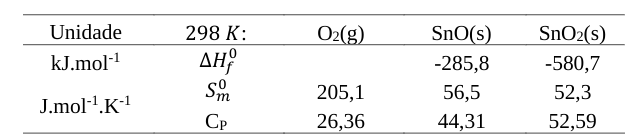
\includegraphics[width=1\linewidth]{2021-07-12-14-57-57.png}
        \end{center}

        \begin{parts}
            \part Obtenha o potencial químico $\mu^0$ de todas as espécies a \SI{298}{\kelvin}.

            \begin{solution}
                Calculamos $\mu^{o}$ a partir das propriedades de formação da espécie:
                $$\mu^0 = \Delta G^0_{f} = \Delta H^0_{f} - TS^0_{m}$$

                \begin{gather*}
                    \mu^0(\ce{SnO2}(s)) = \num{-580,7} - (298 \times \num{52,3} \times  10^{-3}) = \SI{-596,3}{\kilo\joule\per\mole}\\
                    \mu^0(\ce{SnO}(s)) = \num{-285,8} - (298 \times \num{56,5} \times  10^{-3}) = \SI{-302,6}{\kilo\joule\per\mole}\\
                    \mu^0(\ce{O2}(s)) = 0 - (298 \times \num{205,1} \times  10^{-3}) = \SI{-61,1}{\kilo\joule\per\mole}
                \end{gather*}
            \end{solution}

            \part Mostre que a reação de redução do \ce{SnO2}(s) não é
            espontânea obtendo e discutindo o significado da constante de
            equilíbrio $K$ da reação a \SI{298}{\kelvin} e \SI{1}{\atm}.

            \begin{solution}

                No equilíbrio,

                \begin{align*}
                    \Delta \mu^0 &= -RT \ln{K}\\
                    &= \mu^0_{prod} - \mu^0_{reag}\\
                    \Delta \mu^0 &= \num{-302,6} + (\num{-61,1} \times \num{0.5}) - (\num{-596,3}) = \SI{263,15}{\kilo\joule\per\mole}
                \end{align*}

                Assim,

                $$\ln{K} = -\dfrac{\num{263,15e3}}{\num{8,314} \times  298} = \num{-106,2} \implies K \approx \num{7,5e-47}$$

                Pelo $\Delta \mu^0$ positivo, sabemos que a reação não é espontânea no sentido direto.

                A dependência de $\Delta \mu^0$ em $T$ e $\ln{K}$ permite que
                analisemos como a espontaneidade da reação muda com mudanças de
                temperatura na vizinhança de \SI{298}{\kelvin}. Nesse caso, o
                $\ln{K}$
                negativo indica que um aumento na temperatura torna o sentido
                direto ainda mais não espontâneo, enquanto uma diminuição o
                torna mais espontâneo.

                Também podemos extender a análise de ensino médio sobre a
                predominância de produtos e reagentes. No ensino médio, vemos
                que $K > 1$ indica predominância de produtos e $K < 1$ indica
                predominância de reagentes, com uma justificativa algébrica.
                Isso faz sentido termodinâmico: para $K > 1$, $\ln{K} > 0$, logo
                $\Delta \mu^0 > 0$ e a reação direta (que forma produtos) é a
                mais favorável. Análogamente, $K < 1$ implica em $\Delta
                \mu^0 < 0$, em qual caso a reação inversa (que forma
                reagentes) é a mais favorável.
            \end{solution}

            \part Calcule a pressão de oxigênio em equilíbrio a \SI{298}{\kelvin} e
            \SI{1}{\atm} considerando que o sistema pode ser considerado ideal.

            \begin{solution}
                Fases condensadas não contribuem para o valor de $K$ (o termo
                em $RT$ delas é constante para $T$ fixo e entra no seu
                $\mu^0$). Assim, temos que
                $$K = \sqrt{\dfrac{P(\ce{O2})}{P(\ce{O2})^0}} = \sqrt{\dfrac{P(\ce{O2})}{\SI{1}{\bar}}}$$
                \begin{align*}
                    P(\ce{O2}) &\approx (\num{7,5e-47})^{2}\\
                    P(\ce{O2}) &\approx \SI{5,625e-93}{\bar}
                \end{align*}
            \end{solution}

            \part Obtenha a constante de equilíbrio dessa reação a \SI{500}{\kelvin} e \SI{1}{\atm}.
            Considere que $C_p$ não varia com a temperatura.

            \begin{solution}
                Usando o $C_p$ dado, calculamos a entropia molar padrão para cada espécie dada
                \begin{gather*}
                    \ce{O2}  \implies S^0m=\int_0^{500}\dfrac{C_p}{T}\dif T\implies S^0m=C_p\ln 500=\num{26.4}\cdot\num{6.2}=\num{163.7}\\
                    \ce{SnO} \implies S^0m=\int_0^{500}\dfrac{C_p}{T}\dif T\implies S^0m=C_p\ln 500=\num{275.2}\\
                    \ce{SnO2}\implies S^0m=\int_0^{500}\dfrac{C_p}{T}\dif T\implies S^0m=C_p\ln 500=\num{326.6}
                \end{gather*}

                Usando a equação da relação da energia livre de Gibbs da reação temos que
                $$ \Delta rG^0=\Delta rH^0-T\Delta rS^0 = 296-\num{9.1} = \SI{285.9}{\kilo\joule\per\mole} $$
                $$ \Delta rS^0=\dfrac{1}{2}(\num{163.7})+\num{275.2}-\num{326.6}=\num{30.4} $$
                e, portanto:
                $$ \Delta \mu^0=-RT\ln(K_p) $$
                $$ \dfrac{\num{-285.94e3}}{\num{8.31}\cdot 500}=\ln(K_p)=\num{-68.8}\implies K_p=\num{1.3e-30}$$

                %$C_p$ constante com a temperatura implica que a derivada de
                %$\Delta H^0$ é constante. Logo, podemos achar sua dependência
                %na temperatura:

                %\begin{align*}
                %    \Delta C_p &= (\dfrac{\delta \Delta H^0}{\delta T})_{P}\\
                %    &= C_p^{prod} - C_p^{reag}\\
                %    \Delta C_p &= \num{44,31} + \num{0,5} \times \num{26,36} - \num{52,59} = \SI{4,9}{\joule\per\mole\per\kelvin}
                %\end{align*}

                %\begin{align*}
                %    \Delta H^0(T) &= \Delta H^0(298) + \int_{298}^{T} \Delta C_p\,T'\dif T'\\
                %    \Delta H^0(T) &= \Delta H^0(298) + \Delta C_p \dfrac{T^{2} - 298^{2}}{2}
                %\end{align*}

                %O $\Delta H^0(298)$ é simples de calcular, é só produtos menos reagentes:
                %$$\Delta H^0 (298)= \num{-285,8} + 0 - (\num{-580,7}) = \SI{294,9}{\kilo\joule\per\mole}$$

                %Assim, podemos construir a equação:
                %$$\ln{\frac{K(500)}{K(298)}} = \frac{1}{R}
                %\int_{298}^{500}\frac{\Delta H^0(298) + \Delta C_p
                %\dfrac{T^{2} - 298^{2}}{2}}{T^{2}}\dif T$$
            \end{solution}

            \part Estime o valor da constante de equilíbrio a \SI{298}{\kelvin} e \SI{3}{\atm}
            considerando que o sistema pode ser tratado como ideal.

            \begin{solution}
                Seja a integral da derivada parcial em relação a pressão:
                $$ \mu = \mu^0+\underbrace{RT\ln(3)}_{c} $$
                $$ \mu_i = \mu^0_i + c , \mu_f=\mu_f^0+c $$
                Como a diferença se mantém constante independente da pressão, i.e.
                $$ \implies \Delta\mu=\Delta\mu^0 $$
                Temos que essa quantidade se conserva.
                Assim sendo, o $K_p$ vai ser igual para qualquer pressão $P$.
            \end{solution}
        \end{parts}

        \question Para a formação de amônia gasosa a partir de \SI{2}{\mole} de
        nitrogênio e \SI{3}{\mole} hidrogênio gasosos a \SI{500}{\kelvin} e \SI{4}{\atm}, o
        diagrama de energias de reação em função da extensão de reação ao
        lado foi construído:

        \begin{center}
            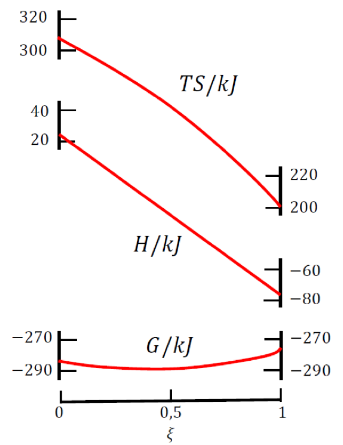
\includegraphics[width=0.5\linewidth]{2021-07-12-15-08-19.png}
        \end{center}

        \begin{parts}
            \part Explique porque a entalpia da reação varia
            linearmente enquanto as outras funções não variam
            linearmente.

            \begin{solution}
                Em delta/H temos uma reação que ocorre linearmente, porque
                conforme há a variação da extensão da reação, teremos uma
                variação diretamente proporcional à variação de entalpia, isto
                é, quanto mais reações ocorrem no sistema, mais energia será
                liberada ou absorvida, diminuindo a entalpia, linearmente.
                Enquanto, por outro lado, o delta/TS que por um lado teria uma
                tendência linear de diminuição energética (pelo número de
                espécies da reação), terá de modo concomitante uma variação
                não-linear do delta/S da mistura, isto posto, a função final
                será não linear e o delta/G terá um ponto de mínimo em
                extensão igual a \SI{0,5} em que a energia livre do sistema será
                mínima.
            \end{solution}

            \part Indique a extensão de reação relacionada à composição
            de equilíbrio nessas condições e calcule o $K_p$.

            \begin{solution}
                A extensão da reação em que teremos o equilíbrio, será o ponto
                0,5, devido ao fato de este ser o ponto de mínimo em delta/G;

                tomando, \ce{N2}(g) + \ce{3H2}(g) $\to$ \ce{2NH3}(g) e sabendo que temos 2
                mols de nitrogênio e 3 mol hidrogênio a ($T = \SI{500}{\kelvin}$ e $atm = 4$),
                o que irá gerar 2 mols de amônia

                Tomemos a fração molar para pegar a pressão total, isto posto
                fração molar:

                Pela extensão da Reação:

                teremos os Ns: 1,5 para Nitrogênio; 1,5 para Hidrogênio; 3 para Amônia

                Calculando as frações molares:
                \begin{gather*}
                    X(\ce{N2}) = 1,5/6\\
                    X(\ce{NH3}) = 3/6
                \end{gather*}

                Seguindo a
                \[ P = P_t \cdot X_n \]

                \begin{gather*}
                    P(N2) = 4atm * 1,5/6\\
                    P(NH3) = 4atm * 3/6
                \end{gather*}

                Dada a expressão de $K_p$,

                $$ K_p=\dfrac{(P_B/P^0)^b}{(P_A/P^0)^a} $$

                Portanto, temos $Kp = P(\ce{NH3})^2/P(\ce{N2})P(\ce{H2})^3 =(\SI{4}{\atm} \cdot
                3/6)^(3/6)/(4atm * 1,5/6)^(1,5/6) (\SI{4}{\atm} \cdot 1,5/6)^(1,5/6) = 4/1$

                Ou seja $K_p = 4$.

            \end{solution}

            \part Esboce  um  diagrama  contendo  as funções termodinâmicas
            para  a  mesma  reação  a  500  K, mas a 10 atm.Inclua no seu
            esboço as funções já apresentadas  para  comparação. Justifique
            sua resposta utilizando derivadas parciais.Identifique   qualquer
            consideração   necessária para a resolução da questão.

            \begin{solution}
            \end{solution}

            \part Considere o efeito na entalpia de mistura $Hmix = Hmix(ideal)+
            HE$, onde HE representa a entalpia de excesso e discuta qual
            seria o efeito na entalpia da reação H, caso os gases
            fossem considerados com  não-ideais. Identifique todas as
            considerações feitas para chegar nessa conclusão.

            \begin{solution}
                Caso os gases não fossem considerados ideias, teríamos também
                uma variação de delta/P que também seguiria uma forma de uma
                solução não ideal, isto é, não seguindo a Lei de Raoult, isto
                é, haveria uma variação não-linear da pressão dos gases do
                sistema. Do seguinte modo:

                \begin{center}
                    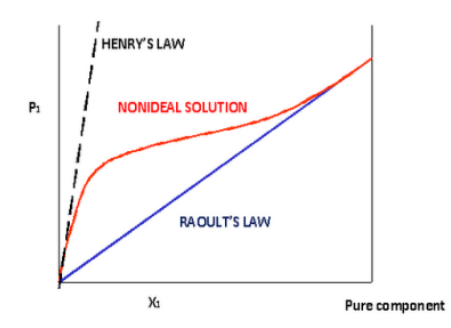
\includegraphics[width=0.5\linewidth]{2021-07-12-17-05-11.png}
                \end{center}

                Pela definição de entalpia, $\dif H \equiv \dif E_{int}+ P\dif
                V+V\dif P$. Teremos então uma variação
                não linear da entalpia do sistema, devido a variação não-linear
                da pressão.

                Assim como, podemos considerar a variação da energia interna do sistema, como sendo dependente do trabalho w, em que para nosso caso, a variação de P.V não será mais linear, podemos esperar também uma variação não linear de w.

                Isto posto, a variação de delta/H não será linear, não somente
                pela variação não linear de parte de suas variáveis, como
                também pelo fato de que são esperadas contribuições da entalpia
                de acesso por conta de interações como as forças de dispersão
                de London ou interações dipolo-dipolo.
            \end{solution}
        \end{parts}

        \question Para a reação 2 Hipitrazolina(aq) = Mauritimato+(aq) +
        Terconozol-(aq), as constantes de equilíbrio do quadro abaixo foram
        medidas em função da temperatura.

        \begin{center}
            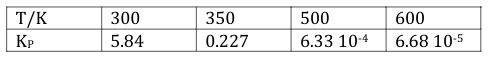
\includegraphics[width=\linewidth]{2021-07-12-15-08-34.png}
        \end{center}

        \begin{parts}
            \part Obtenha os valores de $\Delta rH^0, \Delta rS^0$ e $\Delta rG^0$ o a \SI{300}{\kelvin}
            considerando que as funções termodinâmicas podem ser
            consideradas constantes com a temperatura, nesse intervalo.

            \begin{solution}
                Para a variação da energia livre de Gibbs padrão a $T=\SI{300}{\kelvin}$:
                $$ \Delta rG^0=-RT\ln K_p=-8.32\cdot 300\cdot \ln(\num{5.84})=\SI{-4.4}{\kilo\joule\per\mole} $$
                Para a variação de entalpia padrão:
                $$ \Delta rH^0 = R\dfrac{T_2\,T_1}{T_1-T_2}\ln\del{\dfrac{K(T_2)}{K(T_1)}} $$
                para $T_1$ e $T_2$ próximos de tal forma que a função possa ser considerada constante. Então, tomando $T_1=\SI{350}{\kelvin} $ e $T_2=\SI{300}{\kelvin}$, temos:
                $$ \Delta rH^0=-8.32\cdot \del{\dfrac{105000}{50}}\cdot\ln\del{\dfrac{\num{5.84}}{\num{0.227}}}=\SI{-56.7}{\kilo\joule\per\mole} $$
                Como $\Delta rG^0=\Delta rH^0-T\Delta rS^0$, então para $T=\SI{300}{\kelvin}$:
                $$ \SI{-4.4}{\kilo\joule\per\mole}=\SI{-56.7}{\kilo\joule\per\mole}-\SI{300}{\kelvin}\Delta rS^0$$
                e, portanto
                $$ \Delta rS^0=\dfrac{\Delta rG^0 -\Delta rH^0}{-T}=\dfrac{-4.4+56.7}{-300}=\SI{-0.17}{\kilo\joule\per\mole\per\kelvin} $$
            \end{solution}

            \part Discuta se a reação é entropicamente ou entalpicamente
            favorável.

            \begin{solution}
                Sendo a entropia negativa, i.e. $-T\Delta r S^0 > 0$, com a
                entalpia também negativa temos que $\Delta rG^0=\Delta
                rH^0-T\Delta rS^0<0$, portanto a
                reação é entalpicamente favorável.
            \end{solution}

            \part Sabendo que a reação acima se torna mais rápida com o aumento
            de temperatura, foi sugerido que a temperatura do reator
            fosse aumentada para produzir mais mauritimato$^+$(aq). Com base
            nos cálculos realizados anteriormente, avalie se vale a pena aumentar
            a temperatura e forneça uma proposta alternativa para aumentar a
            produção de mauritimato$^+$(aq).

            \begin{solution}
                Com o aumento de temperatura $\Delta r G^0$ decresce,
                o que torna a reação mais favorável e mais rápida.
            \end{solution}

            \part O que acontece com o equilíbrio estudado se uma
            quantitade apreciável de nitrato de sódio for adicionada ao reator?
            (Considere que os sais de mauritimato$^+$, terconozol$^-$ e que a
            hipitrazolina não precipitam ou interagem com o nitrato de sódio).
            Justifique.

            \begin{solution}
                Considerando que os sais do sistema não reagem ou interagem com
                nitrato de sódio, então a adição de substância não causaria
                interferência diretamente ao equilíbrio. No entanto, caso o
                nitrato de sódio saturasse a solução aquosa a ponto de
                precipitar hipitrazolina, então o equilíbrio seria desfeito
                pois a parte sólida da hipitrazolina conseguiria se dissociar
                nos sais maritimato$^+$ e terconozol$^-$.
            \end{solution}

            \part Esboce no mesmo gráfico o potencial químico da reação
            em função da extensão da reação para 300 e \SI{600}{\kelvin} (você pode
            querer calcular o valor de $\Delta rG^0$ a \SI{600}{\kelvin} para
            ser mais exato, mas não
            é necessário).

            \begin{solution}
            \end{solution}
        \end{parts}

        %\appendix

        %\begin{lstlisting}
        %\end{lstlisting}

    \end{questions}
\end{document}
